Giai đoạn tiền xử lý dữ liệu gồm ba giai đoạn chính: phân tích khám phá dữ liệu, tiền xử lý dữ liệu tiếng Anh, dịch dữ liệu tiếng Anh sang tiếng Việt, ghép từ tiếng Việt. Ngoài ra nhóm cũng xây dựng bộ tiền xử lý dữ liệu tiếng Việt để có thể dùng trong thực tế.

\subsubsection{Phân tích khám phá dữ liệu - EDA (\textit{Exploratory Data Analysis})}
Số lượng bình luận mỗi nhãn được thể hiện dưới dạng barplot ở hình [ref]. Như có thể thấy, các đánh giá được chia ra thành 6 cột tương ứng gồm ``toxic'', ``severe\_toxic'', ``obscene'', ``threat'', ``insult'', ``identity\_hate''. Có thể thấy ``toxic'' chiếm số lượng lớn nhất do đây là tiêu chí chung để có thể đánh giá cho bình luận, các thuộc tính khác có thể xem như là mở rộng hoặc bổ sung chi tiết cho thuộc tính ``toxic''.

\begin{figure}[htb!]
    \centering
    \begin{subfigure}[t]{0.3\textwidth}
        \centering
        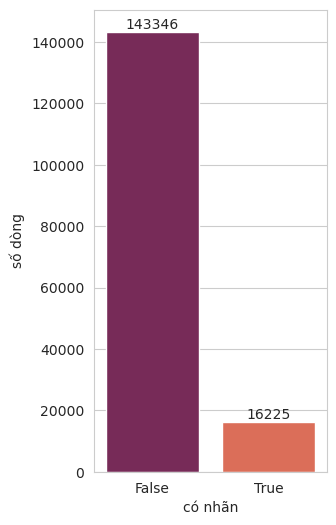
\includegraphics[width=\textwidth]{image/number_of_records_has_label.png}
        \caption{Số lượng bình luận tiêu cực (có nhãn) và không tiêu cực}
    \end{subfigure}%
    \begin{subfigure}[t]{0.7\textwidth}
        \centering
        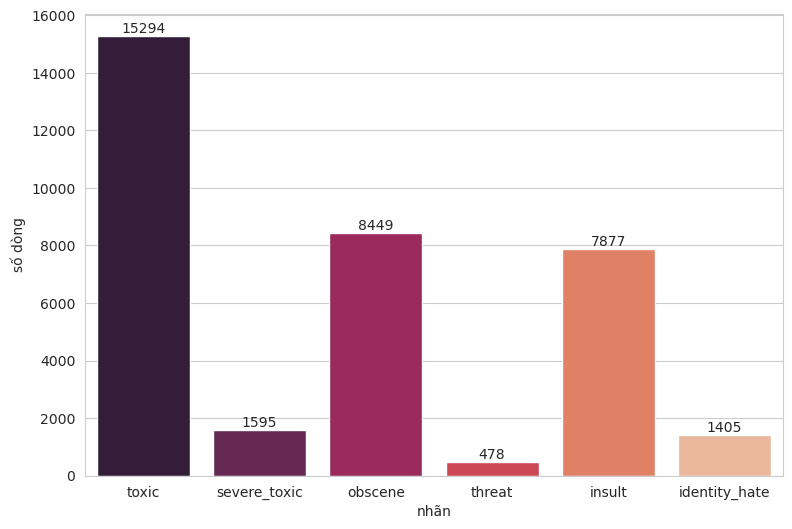
\includegraphics[width=\textwidth]{image/num_records_per_label.png}
        \caption{Số lượng bình luận tiêu cực theo từng nhãn}
    \end{subfigure}\\
    \begin{subfigure}{0.6\textwidth}
        \centering
        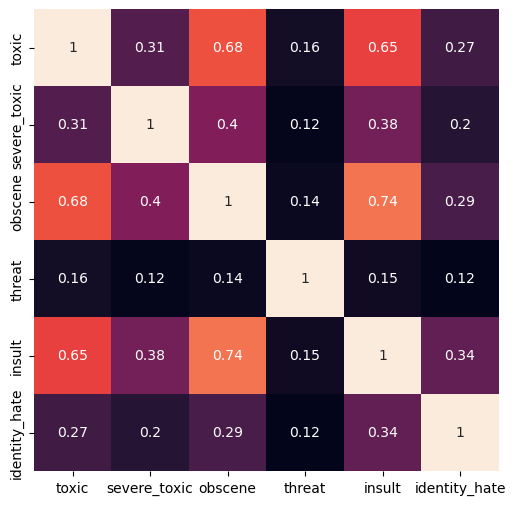
\includegraphics[width=\textwidth]{image/labels_corr.png}
        \caption{Tương quan giữa các nhãn}
    \end{subfigure}%
    \caption{Tương quan giữa số lượng bình luận và nhãn trong tập dữ liệu}
    \label{image:number_of_records_and_labels}
\end{figure}

Chúng ta có thể thấy rằng dữ liệu sạch chiếm đa số trong tập dữ liệu, trong khi dữ liệu độc hại chiếm phần nhỏ hơn. Tuy vậy tỉ lệ dữ liệu độc hại không quá thấp, hoàn toàn có thể sử dụng để huấn luyện mô hình. Dựa vào hình \ref{image:number_of_records_and_labels} về tương quan giữa các nhãn với nhau, chúng ta có thể nhìn ra được sự tương quan lớn ở một số nhãn. Có 3 cặp nhãn có độ tương quan cao mà có thể được chỉ ra ở đây: cặp ``toxic'' - ``obsence'', cặp ``toxic'' - ``insult'' và cặp ``obscene'' - ``insult''.

Dựa vào các mối tương quan trên, có thể đưa ra một số kết luận như sau:

\textit{Ngôn ngữ độc hại thường được dùng trong khi xúc phạm người khác, và khi làm như vậy họ có xu hướng sử dụng ngôn từ thô tục.}

Với kết luận này, có thể dự đoán rằng mô hình được huấn luyện có khả năng bắt được những từ ngữ tục tĩu với độ nhạy tốt.

\subsubsection{Tiền xử lý dữ liệu tiếng Anh}\label{english-preprocess}
Vì dữ liệu là các bình luận trên Wikipedia, nên có một vài điểm đặc biệt trong các bình luận này so với các bình luận thông thường trên các nền tảng khác, ví dụ như địa chỉ IP, các phím tắt (\textit{shortcuts}) của Wikipedia [ref],\dots Nhóm đã đề xuất một chuỗi các thao tác xử lý nhằm giảm bớt các chuỗi không cần thiết, cũng như chuyển đổi các ký tự đặc biệt thành các từ ngữ để máy có thể hiểu được. Chuỗi thao tác như sau:
\begin{enumerate}
    \item Chuyển các địa chỉ IP thành chuỗi \texttt{(ip address)}.
    \item Chuyển các email thành chuỗi \texttt{(email)}.
    \item Chuyển các đường dẫn thành chuỗi \texttt{(url)}.
    \item Chuyển các thời gian (định dạng HH:mm và HH:mm:ss) thành chuỗi \texttt{(time)}.
    \item Chuyển các cụm từ viết tắt trong tiếng Anh (contractions) thành dạng hoàn chỉnh. (bảng \ref{table:english-contractions})
    \item Chuyển các phím tắt của Wikipedia thành chuỗi \texttt{(wikipedia shortcut)}, \\\texttt{(wikipedia namepsace)}, \texttt{(wikipedia file namespace)}.
    \item Chuyển các emoticons thành tên. (bảng \ref{table:emoticons})
    \item Chuyển các emojis thành tên. (bảng \ref{table:emojis})
    \item Xoá tất cả các ký tự đặc biệt, chỉ giữ lại các ký tự có tên khối unicode (\textit{unicode block}) thuộc (``Latin'', ``Greek'', ``Phonetic'', ``Spacing'', ``General Punctuation'', ``Currency Symbols''). (bảng \ref{table:unicode-blocks})
    \item Xoá tất cả các ký tự đặc biệt, chỉ giữ lại các ký tự có tên nhóm unicode (\textit{unicode general category}) thuộc (``L'', ``M'', ``N'', ``P'', ``S'', ``Z'', ``C''). (bảng \ref{table:unicode-categories})
    \item Chuyển tất cả các ký tự đặc biệt còn lại thành các ký tự thuộc bảng mã ASCII. (bảng \ref{table:deunicode})
    \item Tách các ký tự đặc biệt xunh quanh từ ra khỏi từ (ví dụ: {\tt .hello,} thành {\tt .\textvisiblespace hello\textvisiblespace,}).
\end{enumerate}

Sau khi áp dụng các thao tác trên, dữ liệu chuỗi sẽ còn lại các từ đơn dạng: số 0-9, chữ cái a-z và A-Z, dấu câu, ký hiệu, và các tổ hợp của chúng. Nhóm đề xuất các bước phân loại thành hai nhóm: nhóm 1 bao gồm số, dấu câu, ký hiệu và các tổ hợp của chúng, nhóm 2 là các từ còn lại. Nhóm các từ còn lại này sẽ được kiểm tra là từ có nghĩa (nằm trong kho từ (\textit{corpus})), nếu là từ không có nghĩa thì sử dụng các bước sau đây kết hợp với thuật toán sửa lỗi chính tả SymSpell [ref] để đưa về dạng đúng nhất có thể.

\begin{algorithmz}[htb]
    \caption{Mã giả sửa lỗi chính tả cho từ $T$, hàm đoán$(\cdot)$ và hàm tách$(\cdot)$ là các hàm trong thuật toán SymSpell}
    \begin{algorithmic}[1]
        \State Thay thế tất cả ký tự đặc biệt bằng khoảng trắng (chỉ giữ lại nhóm unicode L và N)
        \Comment \texttt{hel+-lo.,wo*/rld} $\to$ \texttt{hel\textvisiblespace lo\textvisiblespace wo\textvisiblespace rld}
        \If {$\left(t\in\text{kho từ}\right)\lor\left[\text{đoán}(t)\in\text{kho từ}\right]$, $\forall t\in T$}
        \Return $T$
        \EndIf
        \Comment \texttt{hello\textvisiblespace orld} $\to$ \texttt{hello\textvisiblespace world}
        \State Xoá các khoảng trắng khỏi $T$
        \Comment \texttt{hello\textvisiblespace world} $\to$ \texttt{helloworld}
        \State Xoá các ký tự bị trùng quá 2 lần khỏi $T$
        \Comment \texttt{hellllo} $\to$ \texttt{hello}
        \State \Return tách$(T)$
        \Comment \texttt{helloworld} $\to$ \texttt{hello\textvisiblespace world}
    \end{algorithmic}
\end{algorithmz}

Mục tiêu của thuật toán trên nhằm giữ lại và trích xuất nhiều thông tin nhất có thể từ những từ vô nghĩa. Đối với các từ có nghĩa, nhóm nhận thấy các ký tự như - (gạch nối), ' (ngoặc đơn),\dots thường không bổ sung ý nghĩa cho từ. Trong nhiều trường hợp nó còn là lỗi sai chính tả (ví dụ như sử dụng dấu câu nhưng không có khoảng trắng: \texttt{hello,word}), hay việc cố tình thêm dấu câu giữa các từ để tránh các bộ lọc thô tục (ví dụ: \texttt{f.u.c.k}). Vì vậy bước 1 của thuật toán trên là thay thế toàn bộ các ký tự đó bằng khoảng trắng. Bước 2, 3 sẽ kiểm tra tính có nghĩa của toàn bộ các từ mới được tạo thành. Trường hợp có nghĩa thì thuật toán dừng lại và trả về các từ có nghĩa; nếu không thường sẽ rơi vào hai trường hợp, hoặc sai chính tả quá nặng (ví dụ: \texttt{hel\textvisiblespace llowo\textvisiblespace rld}), hoặc là các dạng spam từ (ví dụ: \texttt{hellooooooooooo}). Vì vậy bước tiếp theo sẽ xoá toàn bộ các khoảng trắng còn lại, sau đó sẽ chống spam bằng cách xoá toàn bộ các ký tự gần nhau bị trùng quá 2 lần\footnote{Trong tiếng Anh, tần suất xuất hiện hai ký tự giống nhau là rất thấp (bản đồ nhiệt \ref{image:english_bigram_frequency}), dẫn đến việc xuất hiện ba ký tự giống nhau cực kỳ thấp (\texttt{tr\underline{ee} \underline{e}nd}). Đối với tiếng Việt chỉ có duy nhất cụm \texttt{oo} là hai ký tự gần nhau có nghĩa, còn lại các cụm \texttt{aa ee dd oo} là do viết sai chính tả hoặc sử dụng bảng mã Telex khi gõ tiếng Việt.}, cuối cùng dùng thuật toán Symspell để tách các từ con ra. (xem kết quả thử nghiệm tại bảng [appendix])

\subsubsection{Dịch dữ liệu tiếng Anh sang tiếng Việt}
Nhóm đã thử các công cụ dịch thuật khác như MyMemory Translator\footnote{https://mymemory.translated.net/} của translated Labs và gpt-3.5-turbo\footnote{https://openai.com/chatgpt/} của OpenAI nhưng các công cụ này đều bị giới hạn số lượng từ có thể dịch trong một ngày (5000 ký tự đối với MyMemory và 200 requests đối với mô hình gpt-3.5-turbo). Nhóm cũng đã tham khảo công cụ dịch Anh-Việt là mô hình envit5-translation\footnote{https://huggingface.co/VietAI/envit5-translation} của VietAI (được xem là tốt hơn Google Translate vào năm 2022[ref]), mô hình này cho ra kết quả dịch rất tốt đối với những câu ngắn và không có ký tự đặc biệt; nhưng đối với những câu đủ dài (> 1000 ký tự), hoặc có quá nhiều ký tự đặc biệt, hoặc dấu câu bị thiếu, thì mô hình tốn rất nhiều thời gian để chạy và cho ra kết quả không thể sử dụng được. Do đó, nhóm quyết định sử dụng công cụ dịch tài liệu của Google Translate, do Google Cloud Translation cung cấp vì độ chính xác chấp nhận được và gần như không giới hạn (10MB một văn bản).\footnote{Thực tế khi nhóm sử dụng file excel (.xlsx), với hai cột là cột ``index'' và cột ``comment\_text'', thì giới hạn là 2MB một văn bản.}

\subsubsection{Ghép từ tiếng Việt}
Tiếng Việt là ngôn ngữ có sử dụng từ ghép nên nhóm đã sử dụng công cụ ghép từ của thư viện Underthesea để ghép các từ ghép (vd: \texttt{Chàng trai 9X Quảng Trị khởi nghiệp từ nấm sò} $\to$ \texttt{Chàng\_trai 9X Quảng\_Trị khởi\_nghiệp từ nấm sò}).

\subsubsection{Tiền xử lý dữ liệu tiếng Việt}
Đối với tiền xử lý dữ liệu tiếng Việt, nhóm dựa trên các bước 2, 3, 7, 8, 9, 10, 12 của bộ tiền xử lý tiếng Anh (xem \ref{english-preprocess}), bỏ các bước 1, 4, 5, 11 vì không phù hợp với ngôn ngữ tiếng Việt và môi trường ứng dụng (các trang Web và các tin nhắn trong Discord). Sau đó tiếp tục dùng thuật toán SymSpell được tinh chỉnh cho tiếng Việt để đưa các từ sai về dạng đúng\footnote{Đối với tiếng Anh, các từ chỉ khác nhau ở ký tự, nhưng đối với tiếng Việt các từ còn khác nhau ở các dấu thanh (\textit{accents}). Nhóm đã thử và nhận thấy, sử dụng từ điển tần suất (\textit{frequency dictionary}) đã bỏ hết dấu thanh, thay vì sử dụng từ điển tần suất thông thường, sẽ cho ra kết quả chính xác hơn khi sửa lỗi chính tả. (xem [appendix])}. Cuối cùng là ghép các từ ghép trong tiếng Việt.
